Using section formula, 
\begin{align}
\vec{P}&=\frac{1}{1+\frac{3}{4}}\brak{\myvec{-2\\-2}+\frac{3}{4}\myvec{2\\-4}}
=\myvec{\frac{-2}{7}\\[1pt] \frac{-20}{7}}
\end{align}
See 
   \figref{fig:chapters/10/7/2/8/vec.png}.
\begin{figure}
   \centering 
 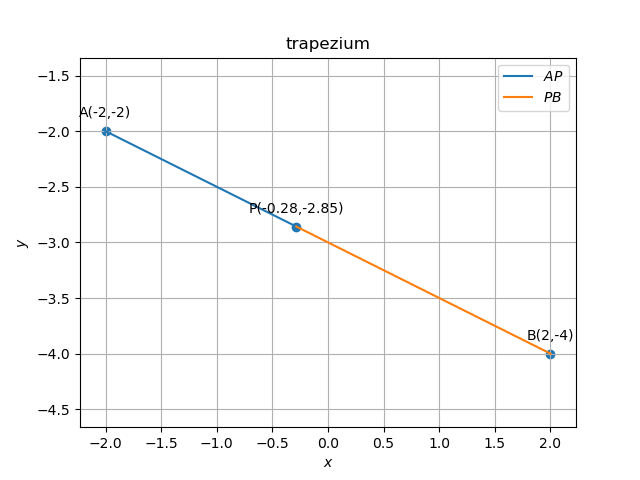
\includegraphics[width=\columnwidth]{chapters/10/7/2/8/figs/vec.png}
   \caption{}
   \label{fig:chapters/10/7/2/8/vec.png}
   \end{figure}
